\section{Introduction}

An operating system is a type of software that acts as an interface between the user and the hardware. It is responsible for handling various critical functions of the computer and utilizing resources very efficiently so the operating system is also known as a resource manager. Various tasks that are handled by OS are file management, task management, garbage management, memory management, process management, disk management, I/O management, peripherals management, etc. \cite{geeksforgeeksHistoryOperating}

\subsection{Advantages of Operating System}

\begin{itemize}
    \item Operating System manages external and internal devices for example, printers, scanners, and other.
    \item Operating System provides interfaces and drivers for proper communication between system and hardware devices.
    \item Allows multiple applications to run simultaneously.
    Manages the execution of processes, ensuring that the system remains responsive.
    \item Organizes and manages files on storage devices.
    \item Operating system allocates resources to various applications and ensures their efficient utilization.

\end{itemize}

\subsection{Disadvantages of Operating System}

\begin{itemize}
    \item If an error occurred in your operating system, then there may be a chance that your data may not be recovered therefore always have a backup of your data.
    \item Threats and viruses can attack our operating system at any time, making it challenging for the OS to keep the system protected from these dangers.
    \item For learning about new operating system can be a time-consuming and challenging, Specially for those who using particular Operating system for example switching from Windows OS to Linux is difficult.
    \item Keeping an operating system up-to-date requires regular maintenance, which can be time-consuming.
    \item Operating systems consume system resources, including CPU, memory, and storage, which can affect the performance of other applications.
\end{itemize}

\newpage
\section{History by Types}

Operating Systems have evolved in past years. It went through several changes before getting its current form. 

\begin{enumerate}
    \item No OS - (0s to 1940s)
    
    Before 1940s, there was no use of OS. Earlier, people are lacking OS in their computer system so they had to manually type instructions for each tasks in machine language(0-1 based language). And at that time, it was very hard for users to implement even a simple task. And it was very time consuming and also not user-friendly. Because not everyone had that much level of understanding to understand the machine language and it required a deep understanding.

    \item Batch Processing Systems - (1950s)
    
    With the growth of time, batch processing system came into the market. Now Users had facility to write their programs on punch cards and load it to the computer operator. And then operator make different batches of similar types of jobs and then serve the different batch(group of jobs) one by one to the CPU. CPU first executes jobs of one batch and them jump to the jobs of other batch in a sequence manner.

    \item Multiprogramming Systems - (1960s and 1970s)
    
    Multiprogramming means more than one program can be active at the same time. It provide user facility to load the multiple program into the memory and provide a specific portion of memory to each program. When one program is waiting for any I/O operations (which take much time) at that time the OS give permission to CPU to switch from previous program to other program(which is first in ready queue) for continuous execution of program with interrupt.

    \item Personal Computers Systems - (1970s)
    
    Unix (1971) revolutionized OS design with simplicity, portability, and multitasking. Personal computers emerged, leading to simpler OSs like CP/M (1974) and PC-DOS (1981).

    \item Introduction of GUI - (1980s)
    
    With the growth of time, Graphical User Interfaces (GUIs) came. First time OS became more user-friendly and changed the way of people to interact with computer. GUI provides computer system visual elements which made user's interaction with computer more comfortable and user-friendly. User can just click on visual elements rather than typing commands. Here are some feature of GUI in Microsoft's windows icons, menus and windows.

    \item Networked Systems - (1990s)
    
    At 1980s, the craze of computer networks at it's peak. A special type of Operating Systems needed to manage the network communication. The OS like Novell NetWare and Windows NT were developed to manage network communication which provide users facility to work in collaborative environment and made file sharing and remote access very easy.

    \item Mobile Operating Systems - (2000s)
    
    Invention of smartphones create a big revolution in software industry, To handle the operation of smartphones , a special type of operating systems were developed. Some of them are : iOS and Android etc. These operating systems were optimized with the time and became more powerful.

\end{enumerate}

\newpage
\section{History by Personal Computer OS}

\subsection{Windows}

Windows is a product line of proprietary graphical operating systems developed and marketed by Microsoft. \cite{wikipediaMicrosoftWindows, wikipediaListMicrosoft}

\begin{figure}[h]
    \centering
    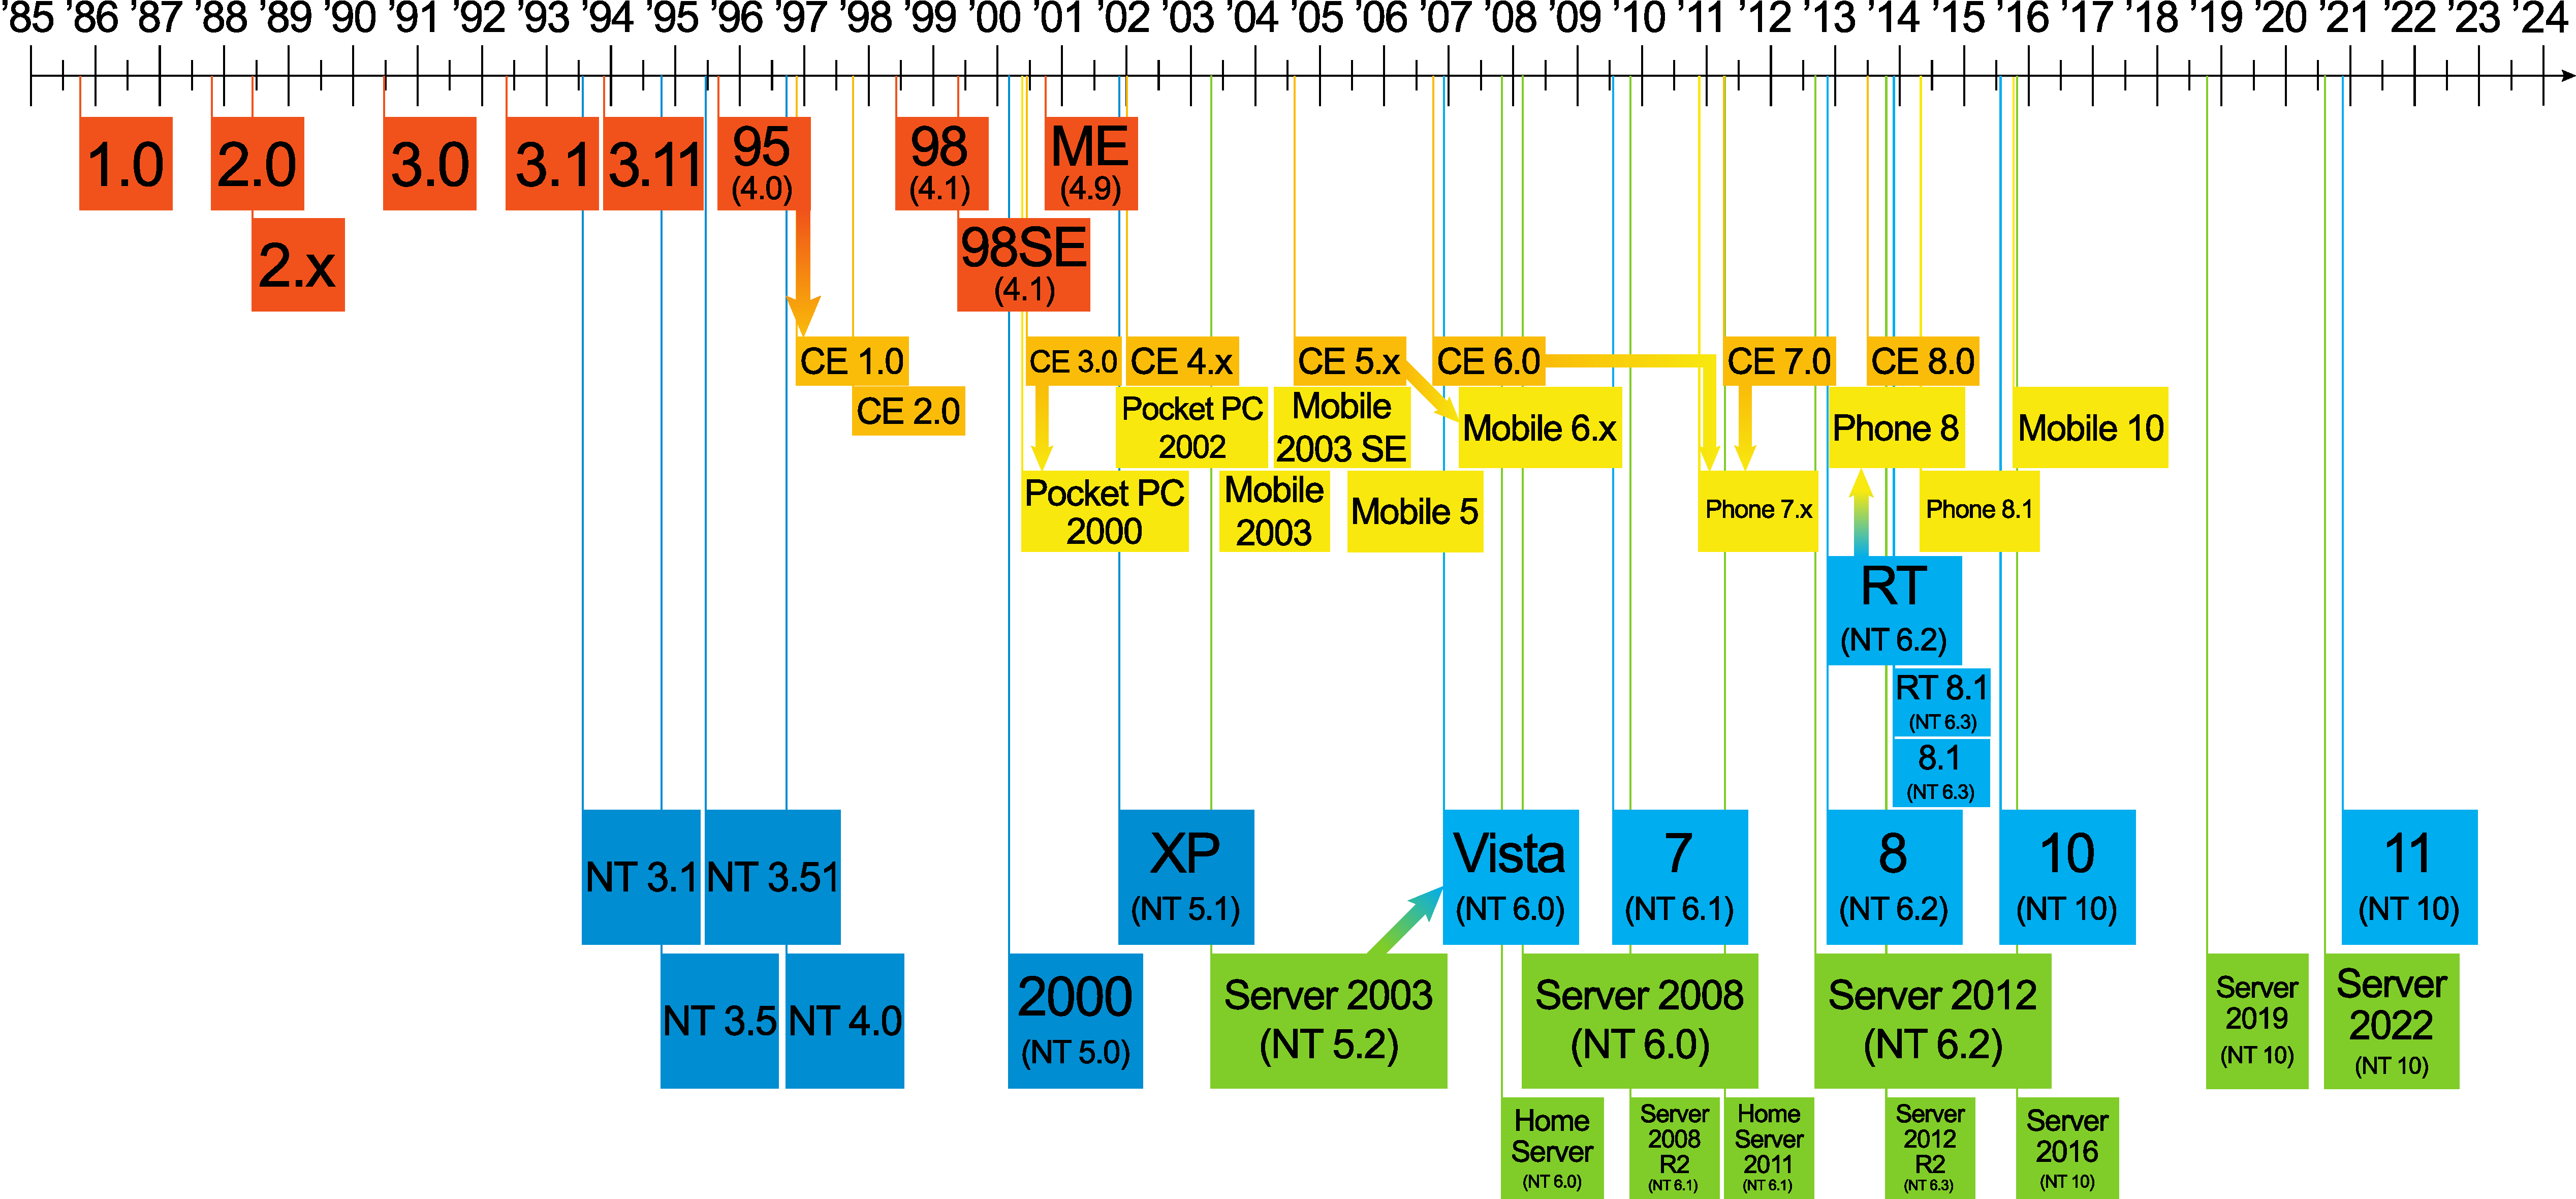
\includegraphics[width=\textwidth]{images/Suite_des_versions_de_Windows}    
    % \vspace{0.5cm}
    \caption{Windows OS Timeline}

\end{figure}



\subsubsection{MS DOS (16bit) Liniage}

\begin{enumerate}
    \item Windows 1.0 (1985) - MS Version 1.0
    \item Windows 2.0/286/386 (1987) - MS Version 2.0
    \item Windows 3.x (1990-1992) - MS Version 3.x
\end{enumerate}

\subsubsection{Windows 95 Lineage (32 bit)}

\begin{enumerate}
    \item Windows 95 (1995) - MS Version 4.0
    \item Windows 98 (1998) - MS Version 4.1
    \item Windows ME (2000) - MS Version 4.9
\end{enumerate}

\subsubsection{Windows NT Lineage (32 \& 64 bit)}

\begin{enumerate}
    \item Windows 2000 (2000) - MS Version 5.0
    \item Windows XP (2001) - MS Version 5.1
    \item Windows Vista (2006) - MS Version 6.0
    \item Windows 7 (2009) - MS Version 6.1
    \item Windows 8/8.1 (2012-2013) - MS Version 6.2/6.3
    \item Windows 10 (2015) - MS Version 6.4
    \item Windows 10 S (2017)
    \item Windows 11 (2021)
\end{enumerate}

\newpage
\subsection{Mac OS}

\textit{macOS}, originally Mac OS X, previously shortened as OS X, is a Unix-based operating system developed and marketed by Apple since 2001. It is the primary operating system for Apple's Mac computers. Within the market of desktop and laptop computers, it is the second most widely used desktop OS, after Microsoft Windows and ahead of all Linux distributions. As of 2024, the most recent release of macOS is macOS 15 Sequoia, the 21st major version of macOS. \cite{wikipediaMacOSVersion, wikipediaMacOSWikipedia, setappFullList}

\subsubsection{MacOS Release Timeline}

\begin{enumerate}
    \item Mac OS X 10.0 Cheetah, March 24, 2001
    \item Mac OS X 10.1 Puma, September 25, 2001
    \item Mac OS X 10.2 Jaguar, August 23, 2002
    \item Mac OS X 10.3 Panther, October 24, 2003
    \item Mac OS X 10.4 Tiger, April 29, 2005
    \item Mac OS X 10.5 Leopard, October 26, 2007
    \item Mac OS X 10.6 Snow Leopard, August 28, 2009
    \item Mac OS X 10.7 Lion, July 20, 2011
    \item OS X 10.8 Mountain Lion, July 25, 2012
    \item OS X 10.9 Mavericks, October 22, 2013
    \item OS X 10.10 Yosemite, October 16, 2014
    \item OS X 10.11 El Capitan, September 30, 2015
    \item macOS 10.12 Sierra, September 20, 2016
    \item macOS 10.13 High Sierra, September 25, 2017
    \item macOS 10.14 Mojave, September 24, 2018
    \item macOS 10.15 Catalina, October 7, 2019
    \item macOS 11 Big Sur, November 19, 2020
    \item macOS 12 Monterey, October 25, 2021
    \item macOS 13 Ventura, October 25, 2022
    \item macOS 14 Sonoma, September 26, 2023
    \item macOS 15 Sequoia, September 16, 2024
\end{enumerate}

\newpage
\subsection{Linux}

Linux is a family of open-source Unix-like operating systems based on the Linux kernel, an operating system kernel first released on September 17, 1991, by Linus Torvalds. It was created by Linus because he felt that the Unix system was lacking, hence he created the linux kernel with the thought \emph{something that he could use at his home}. Torvalds made his personal mascot a penguin named “Tux,” which became a recognizable symbol for Linux around the world. \cite{wikipediaLinuxWikipedia, mitLinusTorvalds}

Linux is the \emph{most widely used operating system} (mainly used in servers and mobile devices like smartphones as Android). When comparing to the general public, windows has the highest market share.

Linux is distributed to the general public as distributions(distros). The most famous being Ubuntu which is based on another distro named Debian. Similarly there are other distributions like Arch Linux, NixOS, Gentoo, Fedora etc. Since the kernel itself is opensource, anyone can create their own disto and distribute it to the general public. Here is a link to a very large image which contains many distributions and their timeline.

\url{https://upload.wikimedia.org/wikipedia/commons/1/1b/Linux_Distribution_Timeline.svg}


\clearpage% or cleardoublepage
\phantomsection
\addcontentsline{toc}{section}{References}
\bibliographystyle{plain}
\bibliography{refernces}